\begin{wrapfigure}{l}{0.5\textwidth}
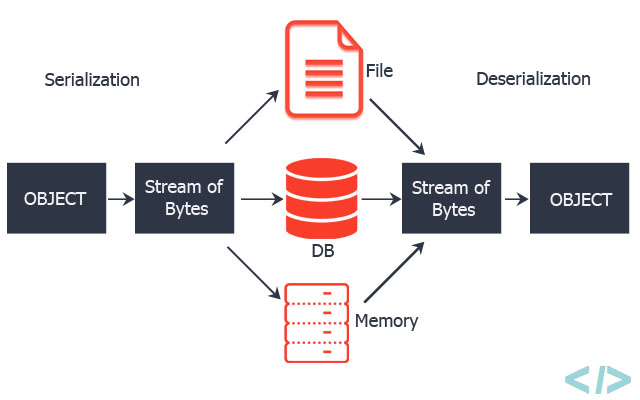
\includegraphics[width=0.3\paperwidth]{header-picture}
\caption*{pc: \href{https://www.codenuclear.com/serialization-deserialization-java/}{codenuclear.com}}
\end{wrapfigure}

Serialization (also known as marshalling) is a powerful data storage technique employed to deal with data that is intended to transmit or store the state of objects in a computer program. During serialization, data structures and objects are converted into a stream of bytes, which then can be stored on a disk or shared over a network. 

Serialization becomes useful when data must be reconstructed via deserialization (or unmarshalling): the serialized stream is used to recreate the original object in memory, and the new object is semantically equivalent to when it was serialized. 

In this lab we will explore a brief history of various serialization techniques and understand how computer files work. Then we will investigate how we can implement these techniques into microcontroller driven systems.

In the following labs, we will actually implement two examples of serialization in ArduinoC and corresponding deserialization. 
